%%%%%%%%%%%%%%%%%%%%%%%%%%%%%%%%%%%%%%%%%%%%%%%%%%%%%%%%%%%%%%%%%%%%%%%
%                                                                     %
%                   Règlement intérieur du Ceten                      %
%                                                                Beta %
%%%%%%%%%%%%%%%%%%%%%%%%%%%%%%%%%%%%%%%%%%%%%%%%%%%%%%%%%%%%%%%%%%%%%%%
%
%  Auteurs :
%    Philippe Becker <philippe.becker@telecomnancy.net
%    Kilian Cuny <kilian.cuny@telecomnancy.net
%    Julien Déoux <julien.deoux@telecomnancy.net>
%    Yoni Lévy <yoni.levy@telecomnancy.net
%    
%  Licence :
%    CC-BY-NC 4.0 (http://creativecommons.org/licenses/by-nc/4.0)
%
%%%

\documentclass{article} % Jusqu'à preuve du contraire, les documents édités par
                                              % le Ceten ne font pas 300 pages.
\usepackage[a4paper,includeheadfoot,margin=2.54cm]{geometry}
\usepackage[francais]{babel} 

\usepackage{hyperref}
\usepackage{graphicx} 
\usepackage{titlesec} 
\usepackage{ifxetex} 
\usepackage[usenames]{xcolor} 
\definecolor{newCeten}{RGB}{130,11,95}
\usepackage{multicol}

\ifxetex
	\usepackage{fontspec} 
	\setmainfont{Roboto Slab}
	\setsansfont{Roboto}
	\setmonofont{Roboto Mono}
	\newfontfamily\condensed{Roboto Condensed}
	\newfontfamily\condensedlight{Roboto Condensed Light}
	\newfontfamily\light{Roboto Slab Light}
	\titleformat*{\section}{\LARGE\condensed\color{newCeten}}
	\titleformat*{\subsection}{\Large\condensedlight\color{newCeten}}
	\titleformat*{\subsubsection}{\large\condensedlight\color{newCeten}}
\else
	\usepackage[utf8]{inputenc} 
	\usepackage[T1]{fontenc} 
\fi

\title{Règlement intérieur}
\author{Philippe Becker \\
	Julien Déoux \\
	Kilian Cuny \\
	Yoni Lévy}
\date\today

%%%%%%%%%%%%%%
%  Document  %
%%%%%%%%%%%%%%

\begin{document}

	\pagenumbering{roman}

	%---------------%
	% Page de garde %
	%---------------%
	
	\begin{titlepage}
		\begin{center}
			
\includegraphics[width=\textwidth]{images/ceten.png}\par
			\vspace{3cm}
			{\Huge \light Règlement intérieur}\par
			\vfill
			{\large Cercle des Élèves de TELECOM Nancy}\par
			{\large \light Association déclarée}
			\vfill
			{\light \today}\par
		\end{center}
	\end{titlepage}
	
	%--------------------%
	% Table des matières %
	%--------------------%
	
	\tableofcontents

	%-----------%
	% Préambule %
	%-----------%
	
	\vfill
	\begin{center}
		{\light Ce règlement intérieur a pour objectif de préciser les statuts
		de l’association Cercle des Élèves de TELECOM Nancy dont l’objet est
		d’aider les élèves adhérents, anciens comme nouveaux, de TELECOM Nancy.
		Il est mis à la disposition de l’ensemble des membres et de tout nouvel
		adhérent.}
	\end{center}
	\vfill

	\clearpage

	%----------%
	% Articles %
	%----------%

	\pagenumbering{arabic}

	\section{Membres}
		
		\subsection{Composition}
			
			L’association se compose de :
			\begin{itemize}
				\item Membres de fait
				\item Membres bienfaiteurs
				\item Membres adhérents
				\item Membres extérieurs
				\item Membres ponctuels
			\end{itemize}

			Toutes ces personnes sont des personnes physiques. Les membres de
			fait ne paient pas de cotisation, sauf s’ils en décident autrement
			de leur propre volonté. Ils n’ont pas accès aux services et
			activités proposés par l’association.

			Les membres bienfaiteurs ne paient pas de cotisation, sauf s’ils en
			décident autrement de leur propre volonté. Ils ont droit de
			participation mais pas de vote aux assemblées générales. Ils n’ont
			pas accès aux services et activités proposés par l’association.

			Les membres adhérents doivent s’acquitter d’une cotisation annuelle.
			Cet acquittement n’est valide que pour l’année scolaire en cours
			(de la date d’adhésion jusqu’au 31 août suivant). Ils ont accès à
			l’ensemble des services et activités proposés par l’association.

			Les membres extérieurs représentent l’ensemble des personnes non
			étudiantes ou alumni de TELECOM Nancy qui souhaiterait rejoindre
			l’association. Ces membres doivent s’acquitter d’une cotisation
			annuelle réduite. Cet acquittement n’est valide que pour l’année
			scolaire en cours (de la date d’adhésion jusqu’au 31 août suivant).

			Les membres extérieurs peuvent uniquement prétendre aux tarifs Ceten
			lors des manifestations organisées par l’association ainsi qu’aux
			avantages liés aux partenariats conclut avec l’association. Ils
			n’ont pas accès aux autres services ou activités de l’association.
			Un membre extérieur n’a pas le droit de participation ni de vote aux
			assemblées générales.

			Les membres ponctuels doivent s’acquitter d’une cotisation à hauteur
			d’un montant défini par le Bureau Des Élèves pour la manifestation
			ponctuelle à laquelle ils participent. Le Bureau Des Élèves se doit
			de lister l’ensemble des membres ponctuels par manifestation. Une
			fois cette manifestation achevée, les membres ponctuels ne sont plus
			membres de l’association. Un membre ponctuel n’a pas le droit de
			participation et de vote aux assemblées générales.

		\subsection{Cotisation}

			Le montant de la cotisation est fixé chaque année par le Bureau Des
			Élèves selon la procédure suivante : les trésoriers peuvent faire
			entendre le montant qu’ils considèrent être le plus juste en
			fonction du besoin financier de l’association, mais ne doivent pas
			oublier le fait que l’association reste composée majoritairement
			d'étudiants. Le Bureau Des Élèves délibère le montant proposé.
			Actuellement, le montant de la cotisation est fixé à 40 euros pour
			l’ensemble des membres adhérents à l’exception des troisième année,
			pour qui le montant de la cotisation s’élève à 25 euros, et des
			adhérents extérieurs pour lesquels le montant de la cotisation
			réduite s’élève à 15 euros.

			Le versement de la cotisation peut être établi par chèque à l’ordre
			de l’association, par liquide ou par carte de paiement et effectué
			au plus tard le 30 du mois de septembre de l’année en cours.
			Toutefois et compte tenu de la situation de chaque adhérent, le
			Bureau Des Élèves se réserve le droit d’accorder un délai
			supplémentaire aux membres qui connaissent des difficultés
			financières. Au-delà de ce délai, le cas par cas est possible auprès
			des Trésoriers du Bureau Des Élèves suite au versement de la
			cotisation et à l’adhésion des statuts. Toute cotisation versée à
			l’association est définitivement acquise. Aucun remboursement de
			cotisation ne peut être exigé en cas de démission, d’exclusion ou de
			décès d’un membre en cours d’année sauf si la démission, l’exclusion
			ou le décès se déroule pendant le mois de septembre de l’année en
			cours.

			Pour tout événement qu’ils organisent, le Bureau Des Élèves et les
			clubs de l’association peuvent réclamer à tous ses participants,
			adhérents de l’association ou non, un chèque de caution d’un montant
			de 200 euros sans lequel la participation à l’événement est
			impossible Dans le cas des membres adhérents de l’association, un
			tel chèque doit être délivré lors de l’adhésion et servira jusqu’à
			sa destruction à la fin de l’année scolaire en cours ou en cas de
			démission, d’exclusion, ou de décès de l’adhérent. 

			Le délai pour remettre ce tel chèque est d’un mois après l’adhésion,
			sous réserve que le membre adhérent ne participe pas entre temps à
			un événement pour lequel une caution est réclamée. Le Bureau Des
			Élèves se réserve le droit de prolonger ce délai si nécessaire, ou
			de retirer le statut de membre en cas de non délivrance du chèque
			après la période donnée. 

		\subsection{Admission des nouveaux membres}
			
			L’association Cercle des Élèves de TELECOM Nancy peut accueillir de
			nouveaux membres à tout moment. Ceux-ci devront respecter la
			procédure d’admission suivante :
			\begin{itemize}
				\item Dans le cas des membres adhérents, l’admission se fait
					suite au versement de la cotisation, de la caution et de
					l’adhésion aux statuts de l’association.
				\item Dans le cas des membres extérieurs, l’admission se fait
					suite au versement de la cotisation réduite et de l’adhésion
					aux statuts de l’association.
				\item Dans les cas des membres de fait et bienfaiteurs, la
					demande se fait tout au long de l’année auprès du Bureau Des
					Élèves qui délibérera au cas par cas.
			\end{itemize}

		\subsection{Exclusion}
			
			Seuls les cas de refus de paiement de la cotisation annuelle,
			infraction aux statuts ou au règlement intérieur de l'association ou
			pour tout autre motif portant préjudice aux intérêts moraux et
			matériels de l’association peuvent déclencher une procédure
			d’exclusion. Celle-ci doit être prononcée par le Bureau Des Élèves à
			une majorité absolue, seulement après avoir entendu les explications
			du membre contre lequel une procédure d’exclusion est engagée. Si
			l’exclusion est prononcée, une procédure d’appel est autorisée.

			Dans le cas d’une procédure d’appel, le membre demandant l’appel
			sera amené à présenter des explications, des témoins et des preuves
			devant le Bureau Des Élèves. La procédure d’exclusion ne sera
			validée que si les deux tiers du Bureau Des Élèves se prononcent en
			faveur de l’exclusion.

		\subsection{Démission}

			Conformément à l'article 7.3 des statuts, le membre démissionnaire
			devra adresser sous lettre simple sa décision au président de
			l’association. Le membre démissionnaire ne peut prétendre à une
			restitution de cotisation sauf si la démission intervient pendant le
			mois de septembre.

	\section{L'Assemblée Générale Extraordinaire}

		Toute Assemblée Générale Extraordinaire se doit de terminer par un point
		“Questions et Réponses du Bureau Des Élèves” dont la durée sera limitée
		au quart du temps total de la réunion, la durée minimale étant d’un
		quart d’heure. %\textcolor{red}{Le but de ce point est de réserver un
		%temps pour que l’ensemble des membres de l’assemblée générale puisse
		%exprimer son opinion sans tenir compte de l’absence du quorum de
		%l’assemblée générale rassemblée à sa cause.}\footnote{Un poil indigeste}
		Il ne faut cependant pas oublier que les membres sont également invités
		à le faire en réunion du Bureau Des Élèves.

	\section{Le Bureau Des Élèves}

			Conformément à l’article 10.4 des statuts de l’association Cercle
			des Elèves de TELECOM Nancy, le Bureau Des Élèves a pour rôle la
			gestion de l'association entre le 1er Janvier de l’année suivant
			leur élection et le 31 Décembre de cette même année, et ce dans le
			but de mettre en œuvre les décisions de la dernière assemblée
			générale et conformément à l'objet des statuts.

		\subsection{Descriptif des postes}

			\subsubsection{Président et Vice-Président}

				Le président est secondé par le vice-président dans toutes ses
				tâches que sont :
				\begin{itemize}
					\item La représentation de l’association dans tous les actes
						de la vie civile.
					\item La représentation de plein droit de l’association
						devant la justice. Il est responsable devant la loi et
						les membres de l’association du bon fonctionnement de
						celle-ci.
					\item La présentation à l’assemblée générale
						ordinaire du rapport moral et du bilan des activités de
						l’association.
					\item La convocation des membres, la rédaction de l’ordre du
						jour et l’animation des réunions.
					\item D’autoriser l’ouverture de comptes bancaires ou
						postaux.
					\item D’assurer en collaboration avec les responsables
						communication la représentation de l’association aux
						différentes structures auxquelles l’association adhère. 
				\end{itemize}

				Il peut donner délégation à un membre du bureau qui sera en
				priorité le vice-président. Il possède le droit de signature sur
				les différents comptes de l'association et sur les contrats
				passés au nom de l’association. En cas d’égalité sur toutes les
				délibérations concernant l’association, en réunion du Bureau Des
				Élèves ou lors d’une assemblée générale du Ceten, la voix du
				président compte double. Il a un accès total aux fichiers
				comptables.

			\subsubsection{Trésorier et Vice-Trésorier}

				Le trésorier est secondé par le vice-trésorier dans toutes ses
				tâches que sont :
				\begin{itemize}
					\item La gestion du patrimoine financier de l’association au
						jour le jour en effectuant les paiements, percevant les
						sommes dues à l’association, encaissant les cotisations.
					\item Le suivi d’une comptabilité régulière pour pouvoir
						estimer au mieux la situation économique de
						l’association et faire des comptes rendus aux autres
						membres du BDE\@.
					\item La présentation à l’assemblée générale ordinaire du
						compte de résultat et du budget prévisionnel.
					\item Le suivi des subventions accordées aux clubs.
					\item Le suivi des demandes de subventions avec le
						président.
					\item La rédaction, en collaboration avec
						les présidents et trésoriers des clubs qui le
						souhaitent, des demandes de subventions comme le Fonds
						de Solidarité et de Développement des Initiatives
						Étudiantes (FSDIE).
				\end{itemize}

				Le trésorier et le vice-trésorier possèdent le droit de
				signature sur les différents comptes de
				l'association. Ils ont un accès
				total aux fichiers comptables. Ils doivent pouvoir rendre compte
				à tout moment de la trésorerie de l’association.

			\subsubsection{Secrétaire}

				Le secrétaire est responsable de :
				\begin{itemize}
					\item La correspondance de l’association.
					\item L’archivage des différents documents.
					\item L’établissement des procès-verbaux des réunions et des
						assemblées générales.
				\end{itemize}

			\subsubsection{Responsable des Clubs}

				Le responsable des clubs est responsable de :
				\begin{itemize}
					\item La liaison directe et privilégiée entre les clubs de
						l’association et le Bureau des Élèves.
					\item Le suivi régulier les clubs de l’association en
						animant des réunions avec les
						présidents des clubs.
					\item L’organisation de formations pour les bureaux.
					\item La gestion des éventuels conflits entre clubs.
					\item La vérification du respect de la Charte des Clubs
						rédigée par le Bureau des Élèves.
				\end{itemize}

			\subsubsection{Responsable Informatique}
				
				Le responsable informatique doit :
				\begin{itemize}
					\item Veiller au bon fonctionnement et à l’entretien du
						matériel informatique ou électronique possédé, loué ou
						mis à disposition du Bureau Des Élèves.
					\item Veiller à la légitimité des programmes et des fichiers
						ainsi qu’à leur mise à jour régulière.
					\item Gérer également les comptes d’impressions et les
						droits d’accès au matériel informatique du Bureau Des
						Élèves.
					\item Veiller à la mise à jour du site du Bureau Des Élèves.
				\end{itemize}

			\subsubsection{Responsable Logistique}

				Le responsable logistique :
				\begin{itemize}
					\item Est le partenaire privilégié entre l’administration de
						TELECOM Nancy et le Bureau des Élèves pour tout ce qui a
						trait aux locaux qui sont sous la responsabilité du
						Ceten. À ce titre, il est primordial que le responsable
						logistique veille au parfait respect des articles qui
						relatent les accords écrits en collaboration avec
						l’administration de TELECOM Nancy concernant la mise à
						disposition et l’utilisation des locaux.
					\item Doit veiller au bon fonctionnement et à l’entretien du
						matériel non informatique possédé, loué ou mis à la
						disposition des membres et des clubs du Ceten.
					\item Est tenu de faire l’inventaire des salles de stockage
						et du matériel alloué aux clubs au moins une fois par
						an.
					\item Doit tenir à jour une liste des équipements mis à
						disposition des clubs.
				\end{itemize}

			\subsubsection{Responsables Communication}

				Le Bureau Des Élèves a deux responsables communications. Leurs
				tâches sont :
				\begin{itemize}
					\item D’assurer les relations publiques internes. À ce
						titre, ils tiennent les membres de l’association au
						courant des événements étudiants.
					\item De s’occuper de la communication entre le Bureau des
						Élèves et les partenaires extérieurs de l’association.
					\item De trouver des partenaires extérieurs afin de
						faciliter l’exécution des objets de l’association.
					\item D’assurer, en collaboration avec le président, la
						représentation de l’association aux différentes
						structures auxquelles l’association adhère. 
				\end{itemize}

			\subsubsection{Responsable des Troisième Année}

				Le poste de responsable des troisième année est une place
				occupée par un élève de troisième année. Il a pour fonction
				d’aider à la passation entre le bureau sortant et le bureau
				entrant. En cela, il est amené à conseiller, suivre et former le
				nouveau bureau.

			\subsubsection{Responsable des Apprentis}

				Le poste de responsable des apprentis est une place occupée par
				un élève apprenti. Il a pour fonction d’assurer le lien entre le
				Ceten et les élèves apprentis tout au long de l’année. Les
				modalités d’élection du responsable apprentis sont les
				suivantes :
				\begin{itemize}
					\item Toutes les promotions d’élèves apprentis doivent être
						réunies afin de faire un vote à main levée pour décider
						du nouveau responsable.
					\item Seuls les élèves apprentis de 1ère et de 2ème année
						sont éligibles à ce poste.
					\item Le bon déroulement de l’élection est à la charge du
						Bureau Des Élèves.
				\end{itemize}

			\subsubsection{Réunion du Bureau Des Élèves}

				Le Bureau Des Élèves se réunit au moins une fois par semaine,
				sur convocation du président, ou sur demande d'au moins trois de
				ses membres. Les décisions sont prises à la majorité absolue des
				voix exprimées. En cas de partage, la voix du président est
				prépondérante. 

				Tout membre dudit bureau qui, sans excuse, n’aura pas assisté à
				trois réunions consécutives pourra être considéré comme
				démissionnaire du Bureau Des Élèves. Les réunions sont ouvertes
				à tous les membres de l’association.

				Il est tenu un compte rendu des séances. Les comptes rendus sont
				signés par le président et le secrétaire. Ils sont établis sans
				blancs ni ratures et conservés au siège de l’association.

				Tout membre de l’association peut, s’il le souhaite, soumettre
				au président de l’association un point à ajouter à l’ordre du
				jour, sous condition que cet ajout soit constructif et non
				contraire au but et au caractère de l’association.

				Le Bureau se réserve le droit d’inviter une personne étrangère à
				l’association, susceptible de l’aider. 

				Le représentant de TELECOM Nancy au BVE du site « Aiguillettes »
				et le représentant du Conseil d’Administration d’Alisé sont des
				invités permanents.

		\subsection{Modalités d’élection du bureau}

			\subsubsection{Conditions d’éligibilité}
					
				Seuls les membres adhérents de l'association, inscrits en
				première ou deuxième année à TELECOM Nancy, majeurs et jouissant
				de leurs droits civiques sont éligibles. Les membres du Bureau
				Des Élèves sont rééligibles s’ils remplissent toujours les
				conditions d’éligibilité.

				Les candidats devront se présenter au sein de listes composées
				selon les modalités de l’article 10.4.5 des
				statuts de l’association. Une
				liste incomplète pourra être déposée. Chaque candidat ne peut
				appartenir qu’à une seule liste.

				Une semaine avant la campagne, les présidents de chaque liste
				doivent déclarer leur liste auprès du président de l’association
				par courrier électronique pour que leur liste soit éligible.
				Libre au président de l’association, en accord avec les
				présidents des listes, de rendre ces déclarations publiques ou
				non.

				Dans l’hypothèse où aucune liste ne serait déposée dans les
				délais impartis, le bureau en place se trouve automatiquement
				reconduit jusqu’à fin janvier ; il organisera une ou plusieurs
				élections dans ce délai suivant les mêmes modalités afin de
				mettre en place un nouveau bureau. A l’issue de ce délai, si
				aucune solution n’a été trouvée, le Président convoque une
				Assemblée Générale Extraordinaire visant à régler la situation.
				Cette Assemblée Générale Extraordinaire siégera et prendra toute
				décision exceptionnellement sans nécessité de quorum.

			\clearpage

			\subsubsection{Organisation des campagnes}

				Durant la semaine avant la campagne, suite à la réception des
				déclarations de listes, le président de l’association organise,
				en collaboration avec les présidents des listes déclarées, une
				réunion de partage des créneaux de campagne. Ce partage sera
				ensuite envoyé à la directrice des études de TELECOM Nancy.

				Avant le début des campagnes, il est possible de mentionner sa
				liste mais interdit d’en faire la promotion ni d'en dévoiler son
				nom. De même, aucune promotion de la liste ne sera tolérée après
				les campagnes. Le président de l’association reste seul arbitre.
				Toute liste qui est jugée non fair-play, qui ne respecte pas les
				règles d’éligibilité et/ou de campagne devra se préparer à des
				sanctions allant de l’avertissement jusqu'à la suppression de la
				liste.

				Les campagnes se déroulent durant deux semaines
				au mois de novembre où les listes déclarées
				organisent des déjeuners, des petits déjeuners, et/ou des
				soirées (extérieure et intérieure).
				
				Le premier midi de la période de campagne est réservé au
				lancement des campagnes en amphithéâtre, c’est-à-dire à la
				présentation des équipes et à la vision des vidéos de campagne.
				Le second midi est réservé à la présentation de leurs
				programmes.

				La date des campagnes est annoncée par voie d’affichage dans les
				locaux de TELECOM Nancy et par courrier électronique au moins
				quinze jours avant leur commencement.

			\subsubsection{Déroulement général des élections}

				Le Bureau des Élèves sortant est responsable du bon déroulement
				de ces élections. Si l'un de ses membres a un intérêt
				particulier dans ces élections, il devra être écarté de leur
				organisation.

				Les élections ont lieu dans la semaine qui suit les campagnes à
				raison d’un tour par jour. Les plages horaires d’ouverture ainsi
				que les localisations précises du bureau de vote seront
				diffusées par voie d’affichage et par courrier électronique au
				plus tard deux jours avant le scrutin. Le bureau en place doit
				tenir les bureaux de vote. Le responsable du bureau de vote est
				le président. Si celui-ci est écarté de l’organisation, c'est un
				membre du Bureau Des Élèves désigné par celui-ci, n'ayant aucun
				intérêt particulier dans ces élections, qui prendra sa place.

				Chaque votant devra présenter une pièce d’identité officielle ou
				sa carte d’étudiant à un membre du Bureau des Élèves et émarger
				sur la liste des adhérents avant de déposer son bulletin dans
				l’urne.

			\subsubsection{Déroulement du dépouillement}

				Au dépouillement, le Bureau des Élèves nomme en plus du
				responsable du bureau de vote, deux assesseurs en son sein. Un
				représentant de chaque liste candidate peut assister au
				dépouillement sans y participer. Le dépouillement a lieu
				immédiatement à la fermeture du scrutin et est organisé par le
				Bureau Des Élèves organisateur des élections.

				Après le dépouillement du scrutin, le président du bureau
				sortant proclame le résultat par affichage et par courrier
				électronique.

		\subsection{Vacances d’un poste - modalités de remplacement}

			En cas de vacance d'un poste (hors président et trésorier de
			l’association), le Bureau doit procéder à son remplacement dans les
			plus brefs délais. Pour cela, une élection sera organisée au sein de
			l'association. Cette élection sera organisée selon les modalités
			suivantes : Dans la semaine qui suit le départ d’un membre de
			l’équipe, le BDE décide d’un éventuel remaniement des postes. Par la
			suite, les membres Ceten auront la possibilité de se présenter pour
			le poste vacant. Les candidats auront la possibilité de faire leur
			promotion durant la semaine suivant ces inscriptions, du lundi au
			jeudi. Par la suite, le vote aura lieu le vendredi, et il n’y aura
			pas de second tour. Dans ce cas précis, il n’est plus tenu de
			respecter la parité 1A/2A.
			
			Lorsqu’un candidat est élu, il s’engage à prolonger son adhésion
			à l’association au moins pour la durée de son mandat, faute de
			quoi le bureau devra remplacer le candidat en suivant
			la procédure décrite ci-dessus.

		\subsection{Remboursement des frais}

			Les membres de l’association ne peuvent recevoir aucune rétribution
			à l'exécution des missions qui leur sont confiées, leur fonction
			étant bénévole. Seuls des remboursements de frais leur sont
			possibles. Ils doivent pour cela faire l'objet d'une décision
			expresse du Bureau Des Élèves, et des justifications doivent être
			produites qui pourront faire l'objet de vérifications.

	\section{Les Clubs}

		Chaque club est une entité interne à l’association, composée uniquement de
		membres actifs et dédiée à un but ou une activité particulière, spécifié lors
		de sa création.	Chaque club a une certaine autonomie d'organisation qui est
		régie par la charte des clubs. Cette charte est déposée et adoptée par le
		Bureau Des Élèves afin de fixer les divers points concernant l’administration
		des clubs. Chaque bureau de club est composé au minimum d’un bureau de club
		de trois personnes composé d’un président, d’un trésorier et d’un secrétaire
		qui doivent signer cette charte. Cette charte peut être modifiée par le
		Bureau Des Élèves. Les bureaux seront alors invités à signer la nouvelle
		charte.

	\section{Utilisation des locaux de la zone élève}
		
		\subsection{Général}

			\subsubsection{Lien avec la Charte de mise à disposition des locaux}

				Le présent article complète et spécifie l’utilisation des locaux
				mis à disposition des membres de l’association Ceten et des
				clubs, en accord avec la charte de mise à disposition des locaux
				proposée par la responsable administrative de TELECOM
				Nancy.

			\subsubsection{Responsables des locaux du rez-de-chaussée}

				Tout responsable doit vérifier au moins quotidiennement, sauf
				mention spécifique, dans la mesure du possible, le respect des
				consignes de sécurité, d’hygiène et de propreté établies par la
				Commission d’Hygiène et Sécurité de l’Université de Lorraine.

				Le bon usage, la vérification du bon état, du bon
				fonctionnement et de la propreté des équipements du local, ainsi
				que la propreté de l’espace et du bon respect des consignes de
				recyclage sont à la charge du responsable de l’espace.

				L’achat de tout nouvel équipement non consommable doit être
				approuvé par le Bureau Des Élèves qui délibérera suite à la
				présentation d’un dossier présentant les raisons d’un tel achat
				ainsi qu’une présentation des devis. Le responsable peut
				déléguer ces tâches.

			\subsubsection{Chauffage et consommation électrique}

				Tous les responsables des locaux sont chargés de vérifier que
				les chauffages de leur local ne fonctionnent pas à plein régime
				lors de la fermeture de l’école. Ils sont aussi chargés de
				vérifier que les appareils informatiques et électroniques dont
				le fonctionnement n’est pas nécessaire et les lumières des
				locaux sont bien éteints.

				En cas de non-respect de ces règles, les responsables concernés
				pourront subir des sanctions allant de l’avertissement à la
				destitution de statut de membre dans le cas le plus grave.

			\subsubsection{Évacuation des poubelles}

				Les responsables sont chargés de porter les poubelles des
				espaces dont ils ont la charge, au sous-sol en empruntant
				l’ascenseur situé dans l’Atrium. Seuls l’espace de travail et la
				cafétéria sont suspendus de cette charge, celle-ci ayant été
				transférée au personnel nettoyant. Dans ces espaces là, si
				l’évacuation des poubelles de la salle n’est pas correctement
				effectuée, le responsable sera prié d’en informer le responsable
				administratif de TELECOM Nancy.

				Les responsables concernés pourront subir des sanctions allant
				de l’avertissement à la destitution du statut de responsable.
				Les sanctions ne seront appliquées que si la majorité absolue du
				Bureau Des Élèves les valident.

			\subsubsection{Note sur l’utilisation des salles}

				Afin de transmettre à l’administration le taux d’occupation de
				l’école le plus précis possible, chaque président de club doit
				notifier l’utilisation qu’il fait des salles une fois par dans
				un rapport d'activité qu'il fera parvenir  à la directrice des
				études de TELECOM Nancy et au Bureau Des Élèves.

		\subsection{Le rez-de-chaussée}
		
		\begin{figure}[]
			\centering
			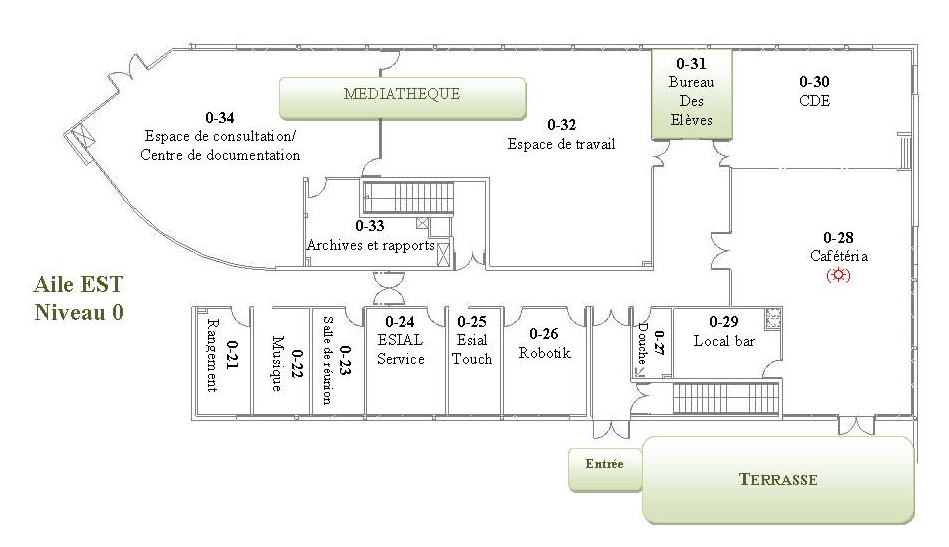
\includegraphics[width=0.8\linewidth]{images/aile_est}
			\caption{Plan du couloir EST rez-de-chaussée (nomination des salles
			non contractuelle)}
			\label{fig:plan}
		\end{figure}

			\subsubsection{La cafétéria (E 0.28 et E 0.30)}

				Le responsable de cet espace est le responsable logistique du
				Bureau Des Élèves. Il travaille en collaboration avec le
				responsable du local Bar, ce dernier étant responsable de
				l’évacuation des déchets de cet espace.

			\subsubsection{Le local du club Bar (E 0.29)}

				Le responsable de cet espace est le président du club Bar.

			\subsubsection{Le Bureau des Élèves (E 0.31)}

				Le responsable de cet espace est le président du Bureau Des
				Élèves.

			\subsubsection{L’espace de travail (E 0.32)}

			Le responsable de cet espace est le responsable logistique du
			Bureau Des Élèves.

			\subsubsection{La douche (E 0.27)}

				Le responsable de cet espace est le responsable logistique du
				Bureau Des Élèves. À ce titre, il doit vérifier, au moins une
				fois par mois ou à chaque transfert de matériel, le bon état et
				la propreté du local.

			\subsubsection{Le local du club Tek’TN (E 0.26)}

				Le responsable de cet espace est le président du club Tek’TN. 

			\subsubsection{Le local du club Studio (E 0.25)}

				Le responsable de cet espace est le président du club Studio. 

			\subsubsection{Le local Telecom Nancy Services (E 0.24)}

				Le responsable de cet espace est le président de Telecom Nancy
				Services. Ce local n’est donc pas sous la responsabilité du
				Ceten.

			\subsubsection{Le local Anim’Est (E 0.23)}

				Le responsable de cet espace est le président de l’association
				Anim’Est. Ce local n’est donc pas sous la responsabilité du
				Ceten. L’achat de tout nouvel équipement commun aux deux
				associations doit être approuvé selon les conditions du Bureau
				Des Élèves et du Conseil d'Administration d’Anim’Est.

			\subsubsection{Le local du club Musique (E 0.22)}

				Le responsable de cet espace est le président du club Musique.

			\subsubsection{Le local Bureau des Sports (E 0.21)}

				Le responsable de cet espace est le président du Bureau Des
				Sports. Ce local n’est donc pas sous la responsabilité du
				Ceten. L’achat de tout nouvel équipement commun aux deux
				associations doit être approuvé selon les conditions du Bureau
				Des Élèves et du Bureau Des Sports.

			\subsubsection{Le centre de documentation (E 0.34)}

				L’association n’est pas responsable de cet espace.

			\subsubsection{Archives et Rapports (E 0.33)}

				Ce local n’est actuellement pas utilisé ou accessible par les
				élèves. En cela, l’association n’est pas responsable de ce
				local.

			\subsubsection{La terrasse}

				Chaque président du club utilisateur de cet espace est
				responsable lorsque son club l’utilise. Tout membre utilisant
				la terrasse pour y cuisiner, manger ou boire est prié de
				laisser le lieu en bon état après son utilisation.

			\subsubsection{Autres espaces}

				Peuvent afficher dans le couloir EST, toutes les personnes qui
				le souhaitent et ayant obtenu l’accord d’un des présidents des
				associations siégeant à TELECOM Nancy. L’affichage ne doit pas
				présenter de caractère discriminatoire ou injurieux.

				Tout non-respect de ces règles entraînera le retrait des
				affiches concernées. Une récidive de la part d’un élève,
				pourtant déjà averti, voulant apposer des affiches à caractère
				discriminatoire ou injurieux sera prise comme une faute et
				celui-ci risque une sanction allant jusqu’à l’exclusion de
				l’association.

				Des armoires sont mises à disposition des clubs dans divers
				lieux du couloir EST\@. Les présidents des clubs utilisant ces
				armoires sont responsables du bon usage, de la vérification du
				bon état, du bon fonctionnement et de la propreté de ces
				armoires. 

				Un double des clés est disponible dans le local du Bureau Des
				Élèves. Tout élève vu en train de forcer les serrures sera
				considéré comme vandale et risque une sanction allant jusqu’à
				l’exclusion de l’association.

				La table d'entraînement du club Tek’TN est située près des
				toilettes de l’aile EST\@. Tout élève vu en train de la
				vandaliser risque une sanction allant jusqu’à l’exclusion de
				l’association. L’utilisation de cette table est placée sous la
				responsabilité du club Tek’TN et plus particulièrement de son
				président.

	\section{Utilisation des locaux hors zone élève}

		\subsection{L’aile Sud-Ouest}

			\subsubsection{L’amphithéâtre (AMPHI SUD)}

				A titre exceptionnel, l’amphithéâtre SUD peut être utilisé par
				les clubs en accord avec l’administration. Chaque président du
				club utilisateur de l’espace est responsable temporaire et doit
				veiller à ce que personne ne mange, ni ne boive un autre
				liquide que de l’eau dans cet amphithéâtre.

			\subsubsection{Les salles de cours (S0.7 à S0.11, S0.13, S1.10 et
			S1.11), les salles de langues (S0.14 et S0.15), la salle d’examen
			(S1.8 et S1.8bis), la salle de rangement (S1.12)}

				Ces salles ne dépendent pas de la responsabilité de
				l'association Ceten.

		\subsection{L’aile Nord}

			En dehors des horaires d’ouverture, cette aile n’est pas accessible
			par les élèves. Les salles qui s’y trouvent ne dépendent pas de la
			responsabilité de l'association Ceten.

		\subsection{L’Atrium}

			Les élèves pourront dans la mesure du raisonnable apposer des
			affiches dans l’Atrium mais seulement au rez-de-chaussée.

	\section{Modification du règlement intérieur}

		Le règlement intérieur de l’association Cercle des Élèves de TELECOM
		Nancy est établi par le Bureau Des Élèves, conformément à l'article 11
		des statuts. Il peut être modifié par le Bureau Des Élèves, sur
		proposition d’un membre de l’association ou d’un membre du Bureau.

		Dans le cas des articles 4 et 5 du règlement intérieur, il peut être
		modifié par le Bureau Des Élèves en accord avec le Directeur de TELECOM
		Nancy, sur proposition d’un membre de l’association ou dudit Directeur.

		La modification se déroule selon la procédure suivante : \\
		Un membre de l’association ou un membre du bureau peut proposer une
		modification au présent règlement lors d’une réunion du Bureau Des
		Élèves qui délibérera de la pertinence de ce changement. Si la majorité
		absolue du bureau vote pour la modification du règlement, celle-ci est
		validée. \\
		Dans le cas des articles 4 et 5 du règlement intérieur, un membre de
		l’association, le directeur de TELECOM Nancy ou un membre du bureau
		peut proposer une modification au présent règlement lors d’une réunion
		du Bureau Des Élèves qui délibérera sur la pertinence de ce changement.
		Si la majorité absolue du bureau et le directeur de TELECOM Nancy
		votent pour la modification du règlement, celle-ci est validée. 

		Le nouveau règlement intérieur sera adressé à chacun des membres de
		l'association par affichage et courrier électronique sous un délai de 7
		jours suivant la date de la modification.

    \vfill
	\begin{center}
		{\large\light Le présent règlement intérieur a été voté lors de la réunion
		du Bureau Des Élèves à Villers-lès-Nancy le 01 février 2016}
	\end{center}
	\vfill
	Signatures\par
	\begin{multicols}{3}
	    \begin{center}
	        Président \\
	        Trésorier \\
	        Secrétaire
	    \end{center}
	\end{multicols}
	\vspace{3cm}
	\clearpage

	\section*{Composition du Bureau Des Élèves}
		
		Il est composé pour l’année 2016 de M. Guillaume HABEN (Président), M.
		Philippe BECKER (Vice-Président), M. Kilian CUNY (Trésorier), M.
		Frédéric GEORGES (Vice-Trésorier), M. Yoni LÉVY (Secrétaire), M. Julien
		DÉOUX (Responsable des Clubs), M. Gauthier DEMANGEON (Responsable
		Informatique), M. Léo JOUËT-PASTRÉ (Responsable Logistique), M. Youri
		KOROSTELEV (Responsable Communication), M. Victor CHOLLEY-BARROYER
		(Responsable Communication), M. Marc PLATINI (Responsable des Troisième
		Année) et M. Thomas DENIS (Responsable des Apprentis).

	\section*{Liste des responsables des espaces}

		Voici la liste des responsables des espaces de 2016 :
		\begin{itemize}
			\item Le local Bureau des Sports (E 0.21) : Claire BILLET
				(Présidente du Bureau des Sports)
			\item Le local Musique (E 0.22) : Quentin TARDIVON (Président du
				club Musique)
			\item Le local Anim’Est (E 0.23) : Matthieu ROUSSELLE (Président
				d’Anim’Est)
			\item Le local Télécom Nancy Services (E 0.24) : Yoni LÉVY
				(Président de Télécom Nancy Services)
			\item Le local Studio (E 0.25) : Eliot GODARD (Président du club
				Studio)
			\item Le local Tek’TN (E 0.26) : Nicolas SCHWARTZ (Président du
				club Tek’TN)
			\item La douche (E 0.27) : Léo JOUËT-PASTRÉ (Responsable
				Logistique du Bureau Des Élèves)
			\item La cafétéria (E 0.28 et E 0.30) : Léo JOUËT-PASTRÉ
				(Responsable Logistique du Bureau Des Élèves)
			\item Le local Bar (E 0.29) : Jérôme CHARREYRE (Président du club
				Bar)
			\item Le Bureau des Élèves (E 0.31) : Guillaume HABEN (Président du
				Bureau Des Élèves)
			\item L’espace de travail (E 0.32) : Léo JOUËT-PASTRÉ (Responsable
				Logistique du Bureau Des Élèves)
			\item Archives et rapports (E0.33) : TELECOM Nancy
			\item L'espace de consultation/centre de documentation (E 0.34) :
				TELECOM Nancy
		\end{itemize}

\end{document}
